%\section{Initial Concept}
%\label{initial-concept}

\paragraph{Initial concept}
In order to develop software the process has to be defined in terms of functions, this is the system's concept.
This section describes how the results of the process analysis (see section \ref{process-analysis}) were transformed to an initial (\ie{} pre-brainstorm) concept.

The initial concept in this project is to develop a system for the \projectdata{} with capability for data request, management, analysis, and security.
Educated guesses were made to find all the parts needed to support these requirements.
Figure \ref{fig:brainstorm-before} describes the full view of the concept. 
The function groups, found in the process analysis and described in figure \ref{fig:research-workflow}, are expanded into: users, external components, data, and functions.

Two direct users and several external users are planned each with their specific set of functions with the data they use and produce.
But also, (offline) external components such as linked and unlinked data, committee protocols, and data administration personnel had to be described.
These components are essential parts of the system but should be provided and are therefore outside of the scope of this study.

Data was planned as follows: the \projectdata{} contains linked clinic and \PRN{} data, but also unlinked data where no match could be found.
This data is the `raw' data of the system.
Raw data may be grouped into subsets which can be analysed resulting in analysis outcomes.
Metadata is used to describe or annotate raw data, which can add meaning or extra information (\eg{} date, file format, etc.).
Provenance and audit data are a result of security measurements, this data is generated by the system and can be used by the data manager to perform security tasks.

Lastly, it is notable that a data request is formulated on the system but the actual approval happens outside of the system.

\begin{figure}[h]
	\centering
	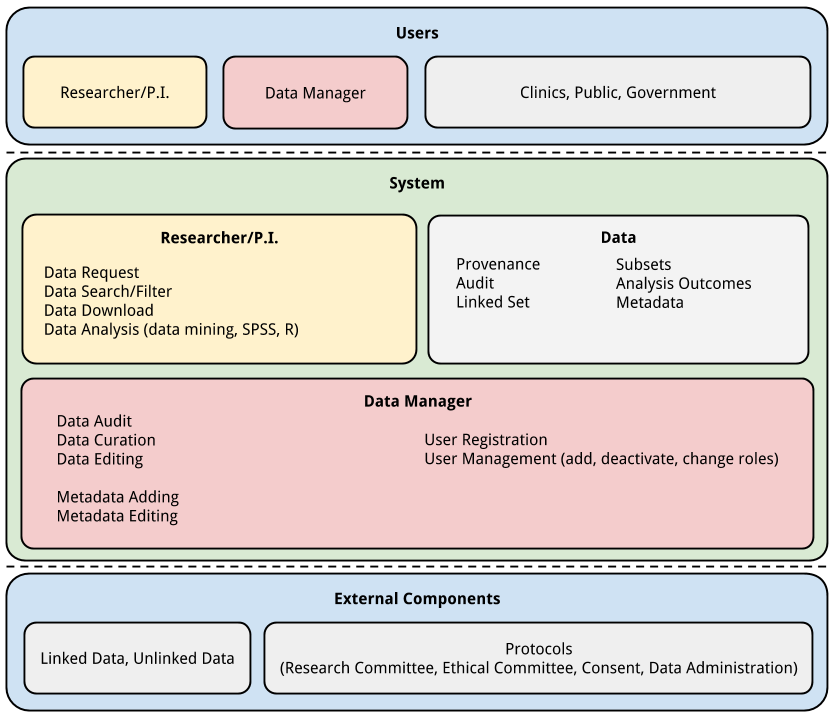
\includegraphics[width=1.0\linewidth]{images/brainstorm-before}
	\caption{
		Initial concept for the \ivfsystem{}, encompassing data and user management. 
		The system offers different sets of functions for three user roles (researcher, data manager, and interested third parties) indicated by colours. 
		External components are (offline) essential parts for system (\eg{} data, regulations) but are outside the scope of development (and by extension of this study).
		Data listed is either available at initialisation of the system or is generated during execution.
	}
	\label{fig:brainstorm-before}
\end{figure}